\section{Characterizing Expert-Parallel Bubbles}
\label{sec:characterization}

We next characterize expert-parallel bubbles and conclude that they are long enough, persistent enough, and predictable enough to schedule fine-tuning work inside.

\subsection{\ac{MoE} models and load imbalance}
An \ac{MoE} model replaces the dense feed-forward network in each transformer block with an \ac{MoE} layer, consisting of $E$ experts and a router that sends each token to its top-$k$ experts~\cite{switch,gshard}.
Large \acp{MoE} commonly combine \ac{TP} for dense computation with \acf{EP} for the experts.
\ac{EP} places different experts on different GPUs and routes individual tokens to the GPUs hosting the appropriate expert (\emph{dispatch})~\cite{deepseekv3,vllm-ep-rfc}.
In a \ac{TP}--\ac{EP} deployment, every GPU observes the same routing decision but executes only its local experts; the expert outputs are then combined across GPUs before the layer computation proceeds (\emph{gather}).

\Cref{fig:anatomy} shows a timeline of one \ac{MoE} layer executing on three GPUs.
Because routing is input-dependent, experts receive different numbers of tokens~\cite{switch,expertchoice,deepseekv3}.
Under \ac{EP}, this results in a per-GPU work imbalance: GPUs hosting more heavily loaded experts finish later, while lightly loaded GPUs finish earlier but cannot proceed as they wait for the processed tokens from other GPUs.
We call this GPU-local waiting interval a \emph{bubble}.
Specifically, a bubble is defined as the interval between completion of a GPU's local expert computation and the dependency that allows the computation to proceed.
We provide additional details on this in \S\ref{sec:appx-arch}.

\Ac{LLM} inference has two phases.
\emph{Prefill} processes the whole prompt and produces the first output token; its latency is measured by \ac{TTFT}, the time from a request's arrival to its first output token.
\emph{Decode} then generates the remaining tokens one at a time; its latency is measured by \ac{TPOT}, the time between consecutive output tokens.
Serving systems enforce \acp{SLO} on both.
In an \ac{MoE} model, the two phases give experts very different amounts of work.
During prefill, all prompt tokens pass through each \ac{MoE} layer in parallel, so expert computation is long and compute-bound.
During decode, each request contributes one token per step, so expert computation is short and memory-bandwidth-bound~\cite{orca,vllm}.
As we show next, this difference determines whether routing imbalance turns into bubbles long enough to leverage for useful work.

\begin{figure}[t]
  \centering
  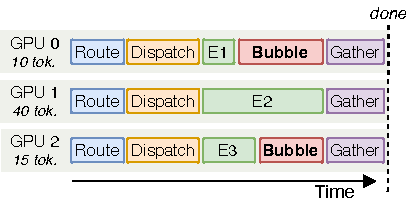
\includegraphics[width=0.82\linewidth]{figures/bubble.drawio.pdf}
  \caption{
    \textbf{Expert-parallel bubbles.}
    Token routing assigns different amounts of expert work
    to different GPUs. GPU~0 finishes its local expert computation (in green)
    before the more heavily loaded GPU~1 but cannot proceed until the
    cross-GPU dependency clears.
    We define this waiting interval (in red) as a \emph{bubble}.
  }
  \Description{
    Two expert-parallel GPUs execute different amounts of local expert
    work. GPU 0 finishes earlier than GPU 1 and waits until the
    cross-GPU dependency clears. This waiting interval is labeled the
    bubble.
  }
  \label{fig:anatomy}
\end{figure}

\subsection{The characteristics of bubbles}
\label{sec:char-obs}

To understand the characteristics of expert-parallel bubbles and how we can best leverage them, we run three experiments and instrument \ac{MoE} layer execution with CUDA events.
We measure, for each GPU and layer, the bubble duration.
For each experiment, we provide key details of the experiment setup, and provide additional details in \S\ref{sec:appx-setup-obs}.

\paragraph{Observation 1: Prefill creates bubbles we can leverage, and that grow
with prompt length.}
\label{sec:char-phase}
\label{sec:char-context}

Routing imbalance occurs during both prefill and decode, but whether a bubble can be leveraged depends on the resulting \emph{absolute} difference in expert computation time across GPUs.
We first measure routing skew, which we define as the most-loaded GPU's routed tokens divided by the mean.
On the \textsc{Qwen3-30B-A3B} model with experts split across two GPUs and no load balancing, and using \textsc{arXiv}-summarization prompts~\cite{cohan-etal-2018-discourse}, we find that this skew is 1.28$\times$ during prefill and 1.75$\times$ during decode.
Thus, token imbalance is more pronounced during decode than prefill on this dataset.
However, because decode expert computation is short, this larger imbalance yields only small bubbles.
Across batch sizes 1--128 and \textsc{arXiv}-summarization prompts of 32--512 tokens in length, while generating 30 tokens per request, the median bubble duration during decode is \SIrange{5}{25}{\micro\second} per layer.
This is insufficient opportunity to effectively schedule work (in \S\ref{sec:design} we use training chunks of \SI{50}{\micro\second}).
When performing prefill with \textsc{arXiv}-summarization prompts of length 8k, in contrast, the bubble length is \SI{0.29}{\milli\second} per layer, which is about 14\% of the layer's expert computation time.
\emph{Thus, prefill offers far more opportunities than decode to schedule work in bubbles.}

The bubble duration during prefill also grows rapidly with the prompt length.
\Cref{fig:lb-sweep} shows the median bubble duration during prefill, for varying prompt lengths, on the \textsc{DeepSeek-V2-Lite} model, with and without load balancing optimizations.
In the \emph{Base} configuration (no optimizations), the median per-layer bubble duration increases substantially when increasing prompt length from 8k to 128k tokens.
The same trend also holds for other \acp{LLM} (\textsc{Qwen3-30B-A3B} and \textsc{Qwen1.5-MoE-A2.7B}, see \S\ref{sec:appx-context}).
\emph{Thus, longer prompts create more opportunities to fill bubbles.}

\paragraph{Observation 2: Load balancing optimizations do not eliminate bubbles.}
\label{sec:char-optimizations}

We next quantify how much bubble duration remains after applying the following three load balancing optimizations.
\begin{enumerate*}[label=(\roman*)]
    \item \Ac{EPLB} uses historical expert loads to place experts and replicate hot ones across GPUs~\cite{deepseekv3,eplb}, giving the runtime multiple expert replicas to which tokens can be sent.
    \item \ac{LPLB}~\cite{lplb} further balances routed tokens across those replicas at dispatch time using linear programming.
    \item \waterfill~\cite{waterfill} assigns shared-expert work to the least-loaded GPUs.
\end{enumerate*}
\waterfill composes naturally with the other two optimizations: \ac{EPLB} and \ac{LPLB} route tokens to physical expert replicas, then \waterfill balances the shared-expert workload.
We therefore also consider their combination.

\begin{figure}[t]
  \centering
  \inputplot{lb_sweep}
  \caption{
    \textbf{Load balancing optimizations reduce bubbles but do not eliminate them.}
    The median per-layer bubble duration on \deepseekmoe, 8$\times$H100 GPUs, and with BF16 precision, for prompts with varying lengths, with and without (combinations of) load balancing optimizations.%
  }
  \label{fig:lb-sweep}
\end{figure}

We evaluate these mechanisms on the \deepseekmoe \ac{LLM} using the \sglang serving engine, 8$\times$H100 with experts split across eight GPUs, and with BF16 precision.
\Cref{fig:lb-sweep} shows the median bubble duration across prompt lengths.
Load balancing reduces the bubble duration substantially compared to \emph{Base} but does not eliminate it.
With prompt lengths of \SI{128}{k}, \emph{Base} exposes \SI{4.79}{\milli\second\per layer}, while \ac{LPLB}, the most competitive load balancing system, still leaves \SI{3.53}{\milli\second} of idle time per layer.
Load balancing is not free either: replicating experts consumes GPU memory, and redistributing tokens at dispatch time can increase communication volume.
For example, \waterfill raises median dispatch time from \SIrange{2.50}{2.65}{\milli\second\per layer} (\SI{6.0}{\percent}); correspondingly, \ac{LPLB}+\waterfill leaves a \SI{3.76}{\milli\second\per layer} bubble, compared to \SI{3.53}{\milli\second\per layer} with \ac{LPLB} alone.
\emph{Thus, minimizing token imbalance by itself does not necessarily eliminate bubbles} and these optimizations must
be weighed against their memory, communication, and runtime overhead.
Lower-precision execution does not close the gap either: our experiments in \S\ref{sec:appx-fp8} show that FP8 leaves the bubble essentially unchanged relative to BF16.

\paragraph{Observation 3: Serving-level colocation systems miss per-GPU bubbles.}
\label{sec:gap}
We next investigate whether existing inference--fine-tuning colocation systems can already exploit the bubbles occurring during prefill.
\llmstation~\cite{llmstation} and \harli~\cite{harli} primarily exploit decode and idle-time underutilization instead of prefill.
\flexllm~\cite{flexllm} and \deltaserve~\cite{deltaserve} can place training work alongside prefill, but only when the serving iteration itself leaves sufficient headroom.
As the prompt length increases, however, GPU compute saturates quickly~\cite{sarathi} and under a stringent serving \ac{SLO}, their planners see little or no capacity in which to admit training.

The limitation is not simply the granularity of their training work.
These systems measure slack once per serving iteration, using signals such as batch composition, iteration latency, predicted request latency, or aggregate engine headroom (see \Cref{tab:colocation_systems} in \S\ref{sec:appx-gap}).
That is reasonable when idle capacity is spread evenly across the GPUs.
\ac{EP}, however, breaks this: within an \ac{MoE} layer, the iteration as a whole looks saturated because it runs at the pace of its most heavily loaded GPU, while the other GPUs finish their experts early and sit idle waiting for it.
A planner with a single headroom budget per iteration cannot see this per-GPU idle time, so it concludes that prefill has no usable capacity even though substantial bubbles remain on individual GPUs. In a trace-driven experiment, a planner that knows the exact mean bubble of each layer but assigns the same budget to every GPU uses only about 1\% of bubble time, whereas planning per GPU from the current routing decision uses 43--45\% (Appendix~\ref{sec:appx-gap}).
Thus, \emph{leveraging expert-parallel bubbles requires a different admission signal}.
The scheduler must estimate slack separately for each GPU at each \ac{MoE} layer, using the current routing decision to determine which GPUs can safely execute work.
